\documentclass[a4paper,12pt]{article} % тип документа

\usepackage{geometry} %геометрия страниц (отступы)
\usepackage[colorlinks=true, linkcolor=blue, urlcolor=blue]{hyperref} %ссылки
\usepackage{subcaption}

%  Русский язык
\usepackage{multirow}
\usepackage{wrapfig}
\usepackage[T2A]{fontenc}			% кодировка
\usepackage[utf8]{inputenc}			% кодировка исходного текста
\usepackage[english,russian]{babel}	% локализация и переносы
\usepackage{graphicx}
\usepackage{todonotes}

% Математика
\usepackage{amsmath,amsfonts,amssymb,amsthm,mathtools}
\usepackage{hyperref}

% графики
\usepackage{pgfplots}
\pgfplotsset{compat=1.9}

\begin{document}

\newgeometry{
    left=2cm,
    right=2cm,
    top=2cm,
    bottom=2cm,
    }
\paragraph{Практикум цифрового производства. Осень 2025}
\section*{Предложение проекта: \newline КВАДРОКОПТЕР С АВТОНОМНОЙ ПОСАДКОЙ}

\paragraph{\underline{Команда}:}
Анатолий Рогов \href{mailto:rogov.ai@phystech.edu}{\underline{rogov.ai@phystech.edu}}, Михаил Мовсесян \href{mailto:movsesian.me@phystech.edu}{\underline{movsesian.me@phystech.edu}}

\paragraph{\underline{Цель проекта}:}
Создать беспилотный летательный аппарат (квадрокоптер), способный совершать автономную посадку в заданную точку, чье положение будет определяться посредством компьютерного зрения.

\paragraph{\underline{Задачи проекта}:}
\begin{itemize}
    \item Разработать и реализовать раму для будущего устройства.
    \item Заказать необходимые технические комплектующие.
    \item Собрать устройство воедино.
    \item Произвести настройки полетного контроллера.
    \item Провести тестирование дистанционного управления.
    \item Изучить особенности работы и возможности библиотеки OpenCV (Python).
    \item Применить компьютерное зрение к квадрокоптеру.
    \item Произвести тестирование посадочного механизма.
\end{itemize}

\paragraph{\underline{Существующие аналоги}:}

\textbf{Open-source проекты}
\begin{enumerate}
    \item \href{https://px4.io}{PX4 Autopilot} (платформа для автономных БПЛА с открытым кодом).
    \item \href{https://ardupilot.org}{ArduPilot} (аппаратно-независимая система управления).
    \item \href{https://www.dji.com/ru}{DJI Tello EDU} (образовательный дрон с программируемым управлением, но закрытой архитектурой).
\end{enumerate}

\paragraph{\underline{Эскиз проекта}:}\

\begin{figure}[h]
    \centering
    \begin{subfigure}{0.4\textwidth}
        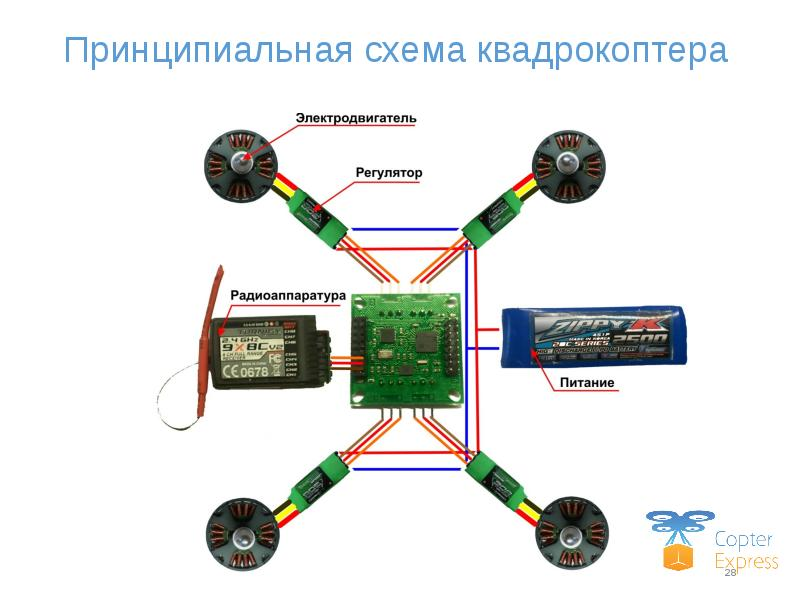
\includegraphics[width=\linewidth]{img/drone.jpg}
    \end{subfigure}
    \hfill
    \begin{subfigure}{0.2\textwidth}
        
\includegraphics[width=\linewidth]{img/opencv.png}
    \end{subfigure}
    \hfill
    \begin{subfigure}{0.2\textwidth}
        
\includegraphics[width=\linewidth]{img/aruco.png}
    \end{subfigure}
\end{figure}

\end{document}
